\chapter{Badania eksperymentalne}
\label{chapter:rezultaty}
\thispagestyle{empty}

W tym rozdziale zostaną przedstawione wyniki badań skuteczności działania aplikacji oraz sposoby ich realizacji. Badania zostaną przeprowadzone w warunkach domowych.

\section{Opis badania}

Badanie ma na celu sprawdzenie skuteczności aplikacji poprzez wykrywanie tonu prostego ze źródła dźwięku znajdującego się w różniej odległości od mikrofonu. Jako generator dźwięku została użyta gitara akustyczna. Badanie zostało podzielone na 3 etapy. W pierwszym etapie zostanie wykorzystany przetwornik elektro-magnetyczny podłączony do komputera na którym uruchomiona jest aplikacja. Połączenie to zrealizowano za pomocą kabla gitarowego. Przewód zakończony jest wtykiem mono jack 6,3 mm. Na gitarze został odgrany jeden dźwięk o częstotliwości 440 Hz. Głośność urządzenia wejściowego, czyli mikrofonu podłączonego do komputera ustawiona jest na 40 db. W tym etapie odległość źródła dźwięku nie będzie miała znaczenia. Wyniki zostały przedstawione za pomocą wykresu słupkowego, gdzie oś X wyrażona jest w centymetrach. Odległość mikrofonu od źródła dźwięku została zwiększana co 40 cm. Oś Y wyrażona jest w  Hz i stanowić będzie średnią arytmetyczną 30 pierwszych pomiarów wysokości tonu prostego w czasie 0.5 sekundy. 

\section{Rezultaty badań}

Etap pierwszy, wyniki podłączenia przetwornika elektro-magnetycznego zamontowanego w gitarze z komputerem, na którym uruchomiona została aplikacja zostały przedstawione na rysunku 4.1.


\begin{figure}[h!]
  \centering
  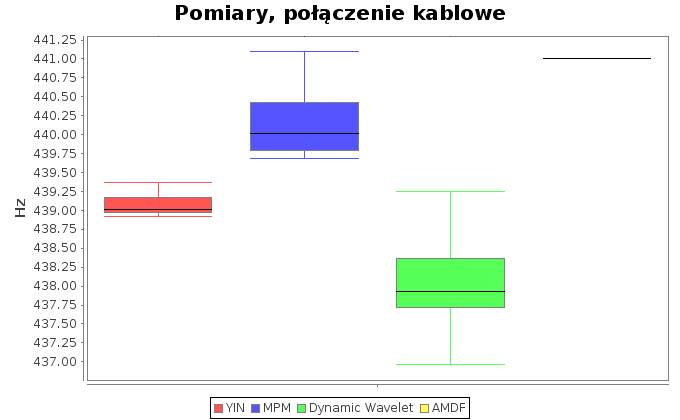
\includegraphics[width=0.5\linewidth]{rys/BoxPlots/kabel}
  \caption{Wykres przedstawiający wyniki połączenia kablowego.}
  \label{fig:schemat}
\end{figure}





Algorytm AMDF we wszystkich pomiarach wskazywał dokładnie 441 Hz, więc te wyniki nie wymagają przedstawienia graficznego. Jak widać na rys 4.1 najmniejsza rozbieżność wartości została zanotowana przy użyciu metody YIN. Natomiast przy użyciu metody Dynamic Wavelet rozbieżność była największa. W przypadku algorytmu MPM mediana wartości osiągnęła częstotliwość 440 Hz. Była to częstotliwość odgrywana na instrumencie.
 
 \newpage
Kolejnym etapem jest wykonywanie pomiarów z zadanej odległości.


\begin{figure}[h!]
  \centering
  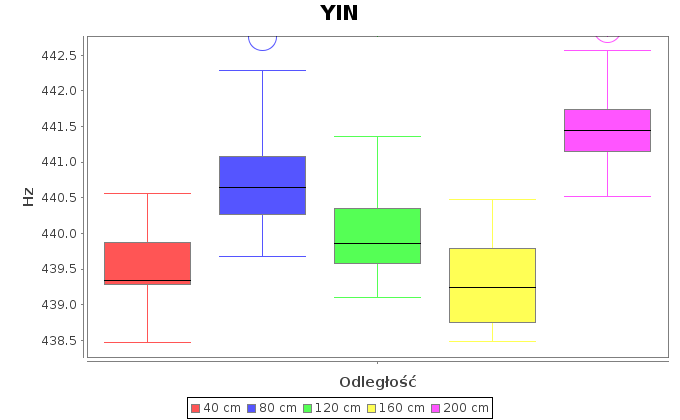
\includegraphics[width=0.5\linewidth]{rys/BoxPlots/YIN_mic_wb}
  \caption{Wykres przedstawiający wyniki przy użyciu algorytmu YIN oraz zastosowaniu mikrofonu wbudowanego.}
  \label{fig:schemat}
\end{figure}


Podczas tego etapu dodatkowym czynnikiem wpływającym na wyniki badań jest odległość, która została podana w opisie badania. Wykorzystany algorytm do przeprowadzenia tego pomiaru to YIN. Jest to pierwszy z czterech wybranych algorytmów. Wybór tego algorytmu został podyktowany przez chęć wykorzystania metody autokorelacji, której użytwa algorytm YIN. Jako urządzenie wejściowe został użyty standardowy wbudowany mikrofon. Jak można odczytać z wykresu na rys.4.2 wartości są zróżnicowane, lecz ich amplituda nie jest większa niż 2 Hz od częstotliwości 440 Hz. Jednak nie są one tak dokładne jak w przypadku połączenia kablowego. Zbiór z którego wyliczona mediana zwraca 440 Hz to zbiór, który powstał poprzez pomiar z odległości 120 cm.


\begin{figure}[h!]
  \centering
  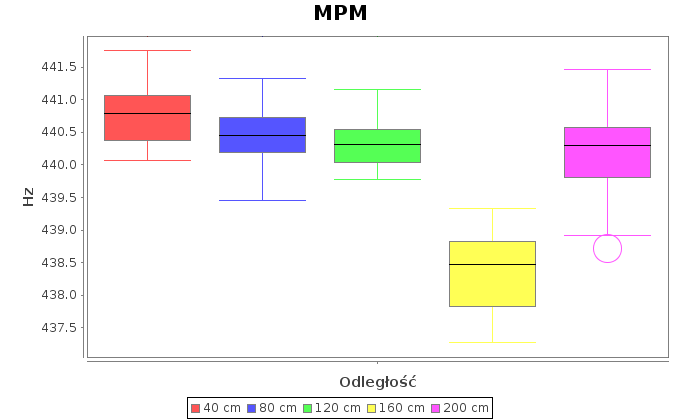
\includegraphics[width=0.5\linewidth]{rys/BoxPlots/MPM_mic_wb}
  \caption{Wykres przedstawiający wyniki przy użyciu algorytmu MPM oraz zastosowaniu mikrofonu wbudowanego.}
  \label{fig:schemat}
\end{figure}


W tym wypadku do wykonania pomiarów został użyty algorytm MPM. Jak w poprzednim przypadku został również użyty standardowy wbudowany mikrofon. Jak można odczytać z wykresu na rys.4.3  wartości z teoretycznie najbardziej dokładnego pomiaru, czyli 40 cm znajdują się w przedziale od 440.4 Hz do 441 Hz. Mediany kolejnych pomiarów są do siebie zbliżone. Wyjątek stanowi wynik pomiaru z odległości 160 cm. Znacznie odbiega od reszty. Strój instrumentu nie mógł ulec zmianie co potwierdza kolejny pomiar z większej odległości  w tym przypadku mógł zadziałać negatywnie na poprawność wyników czynnik jakim są zakłócenia występujące podczas pomiaru.


\begin{figure}[h!]
  \centering
  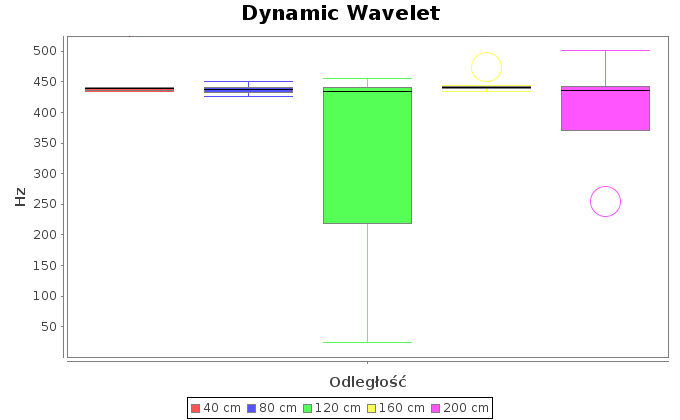
\includegraphics[width=0.5\linewidth]{rys/BoxPlots/Dynamic_mic_wb}
  \caption{Wykres przedstawiający wyniki przy użyciu algorytmu Dynamic Wavelet oraz zastosowaniu mikrofonu wbudowanego.}
  \label{fig:schemat}
\end{figure}

\newpage
Kolejny pomiar dotyczy wykorzystania algorytmu Dynamic Wavelet. W tym przypadku również jak w dwóch poprzednich został użyty ten sam mikrofon jako urządzenie wejściowe. Jak można odczytać z wykresu na rys.4.4 rozbierzność wyników pomiaru z odległości 120 cm spowodowała przeskalowanie wykresu. W tym wypadku również dużą rozbieżnościa charakteryzuje się pomiar z odległości 200 cm. Reszta pomiarów oscyluje wokół częstotliwości 440 Hz.


\begin{figure}[h!]
  \centering
  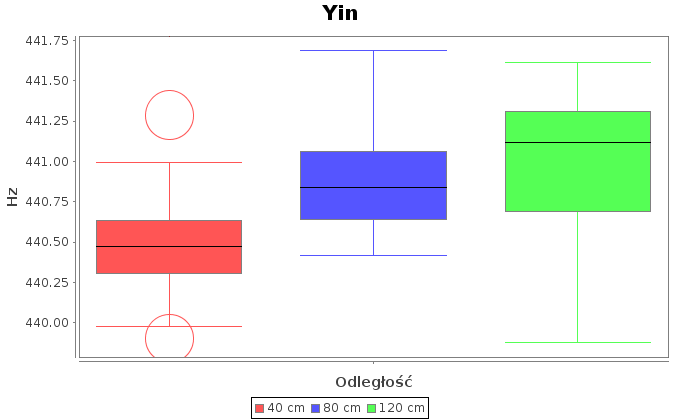
\includegraphics[width=0.5\linewidth]{rys/BoxPlots/YIN_mic_zew}
  \caption{Wykres przedstawiający wyniki przy użyciu algorytmu YIN oraz zastosowaniu mikrofonu zewnętrznego.}
  \label{fig:schemat}
\end{figure}


\newpage
Podczas kolejnego zbioru pomiarów został użyty algorytm YIN, jednakże z mikrofonem zewnętrznym. Przedstawiony wykres na rys. 4.5 zawiera jedynie 3 odległości z powodu tego, iż nie sprawdził się na większe odległości i kolejne próby jej zwiększania dawały winik równy zero. Wszystkie pomiary mieszczą się w granicach od 440 Hz do 441 Hz, co można uznać za satysfakcjonujący wynik.


\begin{figure}[h!]
  \centering
  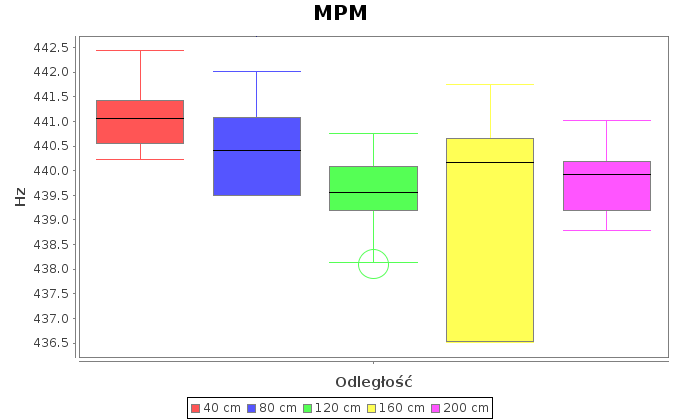
\includegraphics[width=0.5\linewidth]{rys/BoxPlots/MPM_mic_zew}
  \caption{Wykres przedstawiający wyniki przy użyciu algorytmu MPM oraz zastosowaniu mikrofonu zewnętrznego.}
  \label{fig:schemat}
\end{figure}


W tym przypadku został ponownie zastosowany algorytm MPM jednak dla uzyskania tych pomiarów użyto mikrofonu zewnętrznego. Algorytm zdecydowanie lepiej poradził sobie z odległością niż jego poprzednik. Jedyny pomiar z dużą rozbieżnością danych to pomiar z 160 cm. Zostało to przedstawione na wykresie na rys. 4.6. Prawdopodobnie wynikał on z zakłóceń występujących podczas dokonywania pomiaru. Do zakłóceń możemy zaliczyć: szum generowany przez wentylator komputera. Mediany pomiarów ze wszystkich odległości oscylują wokół częstotliwości 440 Hz, czyli oczekiwanej.



\begin{figure}[h!]
  \centering
  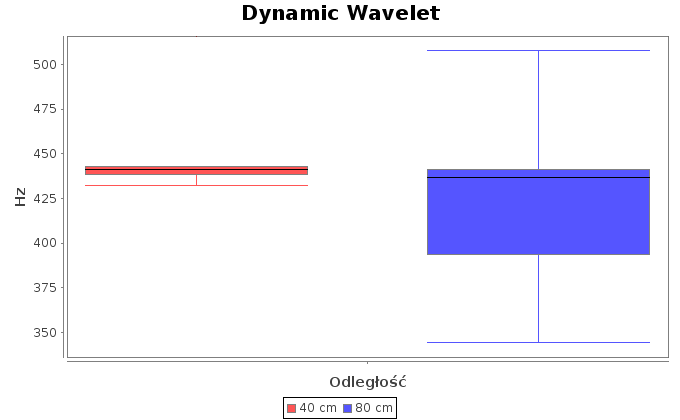
\includegraphics[width=0.5\linewidth]{rys/BoxPlots/Dynamic_mic_zew}
  \caption{Wykres przedstawiający wyniki przy użyciu algorytmu Dynamic Wavelet oraz zastosowaniu mikrofonu zewnętrznego.}
  \label{fig:schemat}
\end{figure}

\newpage
Ostatnim z przedstawionych wykresów jest wykres na rys 4.7, który obrazuje pomiary wykonane przy użyciu algorytmu Dynamic Wavelet oraz mikrofonu zewnętrznego. Na tym wykresie zostały przedstawione tylko dwa zbiory pomiarów. Z odległości 40 oraz 80 cm. Przy większej odległości wynik wynoził 0. Przy pierwszej odległości wynoszącej 40 cm. Mediana, jak i wszystkie pomiary z wyjątkiem wartości skrajnej są w przedziale od 440 Hz do 441 Hz. Taki wynik jest zadowalający. Przypadku tej konfiguracji tj. algorytmu Dynamic Wavelet oraz mikrofonu zewnętrznego można zauważyć coraz większą rozbieżność wyników.


Na koniec warto wspomnieć o algorytmie AMDF. Nie zostały zamieszczone wykresy oraz tabele z dokładnymi pomiarami przedstawiające wyniki tego algorytmu, ponieważ we wszystkich pomiarach rezultat wynosił 441 Hz.

Podsumowując przeprowadzone badania, można wywnioskować, iż działanie aplikacji jest jak najbardziej satysfakcjonujące. Wszystkie pomiary zostały wykonane w warunkach domowych, co może mieć znaczący wpływ na wyniki poszczególnych algorytmów. Wpływ mogą mieć również przypadkowo wygenerowane zakłócenia z otoczenia.
